227. На гранях кубика написаны 6 натуральных чисел, три из которых видны на рисунке. Известно, что произведение чисел, написанных на противоположных гранях, одинаковы. Какое наименьшее значение может принимать сумма всех чисел на гранях кубика?
\begin{center}
\begin{figure}[ht!]
\center{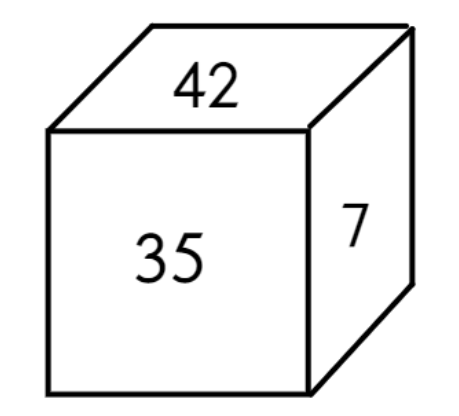
\includegraphics[scale=0.25]{02.png}}
\end{figure}
\end{center}
